\documentclass[12pt, a4paper, oneside]{article}
\usepackage{amsmath, amsthm, amssymb, bm, graphicx, hyperref, mathrsfs,color}

\begin{document}

%\maketitle
\begin{center}
	\rule{\textwidth}{1pt}\par
	\vspace{5mm}
	{\large\scshape UM-SJTU Joint Institute}\\[\baselineskip]
	{\large\scshape Physics Laboratory}\\
	(Vp241)
	\rule{\textwidth}{1pt}\par
	\vspace{4cm}
	{\large\scshape Laboratory Report}\\[\baselineskip]
	{\large\scshape Excercise 3}\\[\baselineskip]
	{\large\scshape Solar Cells: I-V Characteristics}\\[\baselineskip]
\end{center}
\vspace{7cm}

\begin{tabular}{lll}
	Name:Kaixuan Wang & ID:523370910219 & Group:11 \\
	Date: {\today}    &                 &         \\
\end{tabular}


\rightline{\footnotesize[rev4.1]}
\pagebreak

\section{Introduction}
% \textcolor{blue}{This part should include a brief description of the experiment: its objectives, underlying physical model and phenomena, and equations that you will use in
% 	your calculations. It may be a bit longer than that below, but you should not simply copy the lab manual or quote long passages from textbooks.}
\indent

Solar energy is becoming more and more popular today because of its low pollution. A key component for solar energy is solar cell, which 
directly transforms the solar radiation into electrical energy.

The objective of this experiment is to get familiar with solar cell and learn something about its current-voltage 
Characteristics and also measure the cell's $fill factor$ and energy conversion efficiency.

\section{Experimental setup}
\indent

\subsection{Equipments used in the experiment}
\indent

Devices used in the experiment include the following: a photovoltaic device (5W), a 300 W tungsten-halogen lamp functioning as 
the source of radiation, two digital multimeters, two adjustable resistors, 
a solar power meter, a wiring board and a measuring tape

\subsection{Measurement procedure}
\indent

In this experiment, we will look into the relationship between the four main configurations of the soalr cell:
$I,V,P,R$. We will study the relationship of I-V,P-V and P-R. We also pay attention to the fill factor and energy conversion efficiency.

We do the following steps in the experiment:
\begin{itemize}
	\item Turn on the light and the fan, and wait until it reaches its working intensity
	\item Design a measuring circuit with the photovoltaic device and connect the elements
	\item Adjust the distance between the light source and the photovoltaic device until proper distance is meter
	\item Do measurements, change the distance between these two devices and repeat measurements
	\item Plot out the desired graph
\end{itemize}

There is one important equation that we want to prove using teh results of experiment:
\begin{equation*}
	V = \frac{n k T}{q} \ln\left(\frac{I_{sc}}{I_0} + 1\right)
\end{equation*}

\section{Measurements and Results}
\subsection{Light Source Power}
\indent

We will need to know the area of the solar cell for further calculations. The data is recorded in the following
tables:

\begin{figure}[htbp]
	\centering
	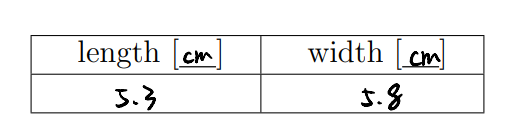
\includegraphics[width=0.9\textwidth]{D1.png}
	\caption{Area of solar cell}
	\label{fig2}
\end{figure}

\begin{figure}[htbp]
	\centering
	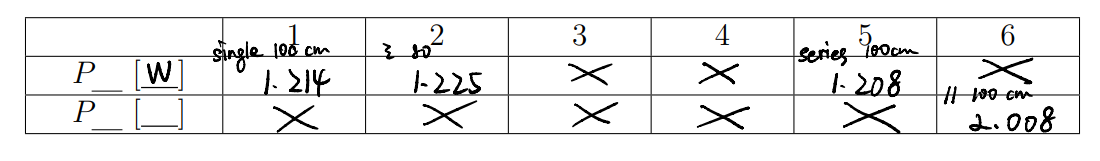
\includegraphics[width=0.9\textwidth]{D2.png}
	\caption{Power of solar cell}
	\label{fig2}
\end{figure}

From the table we can see that the area of the cell should be 30.74$cm^2$. And the corresponding power is 
shown in the data table.

\subsection{I-V Characteristics without Load Resistance}
\indent

We here use a digital multimeter to calculate and measure the I-V characteristics without load resistance. The results
are shown in the following table:
\begin{figure}[htbp]
	\centering
	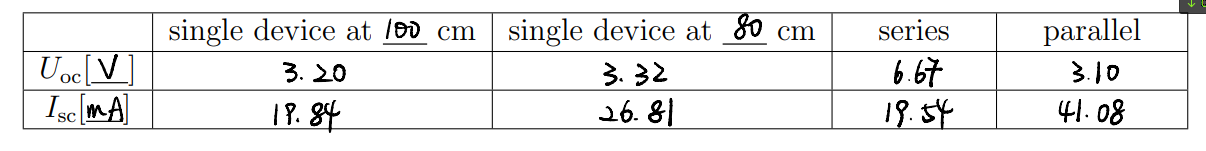
\includegraphics[width=0.9\textwidth]{D3.png}
	\caption{I-V Characteristics Without Load Resistance}
	\label{fig2}
\end{figure}

\subsection{I-V Characteristics with Load Resistance}
\indent

Here we add a load resistance to the circuit for further calculation and study. For each of the four situations
mentioned above, we change the value of resistance and take 20 groups of data for each situation. The data are given 
in the following charts:

\begin{figure}[htbp]
	\centering
	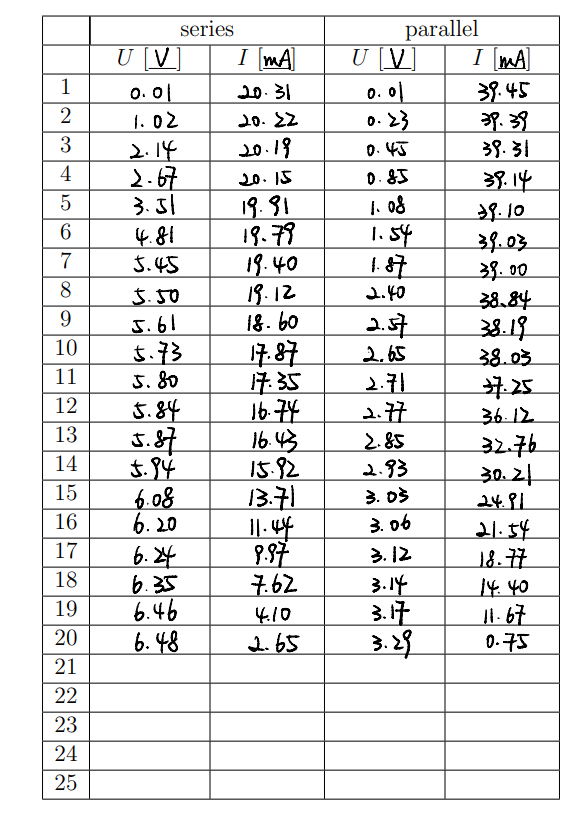
\includegraphics[width=0.9\textwidth]{D4.png}
	\caption{I-V Characteristics with Load Resistance}
	\label{fig2}
\end{figure}

\begin{figure}[htbp]
	\centering
	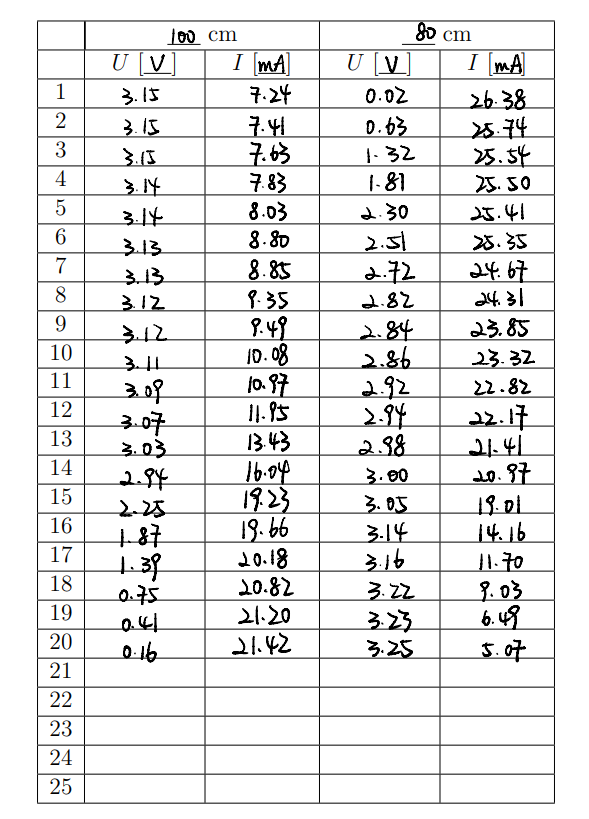
\includegraphics[width=0.9\textwidth]{D5.png}
	\caption{I-V Characteristics with Load Resistance}
	\label{fig2}
\end{figure}

All the data are presented in the tables above with the situations indicated at the heading of the charts.
All there data will be plotted in one single figure together later in the next subsection.

\subsection{I-V Curve}
\indent

Using the data acquired from the foru situations given above, we plot all four of them into one single graph
to show the relationship between I and V. The graph is given as following:

\begin{figure}[htbp]
	\centering
	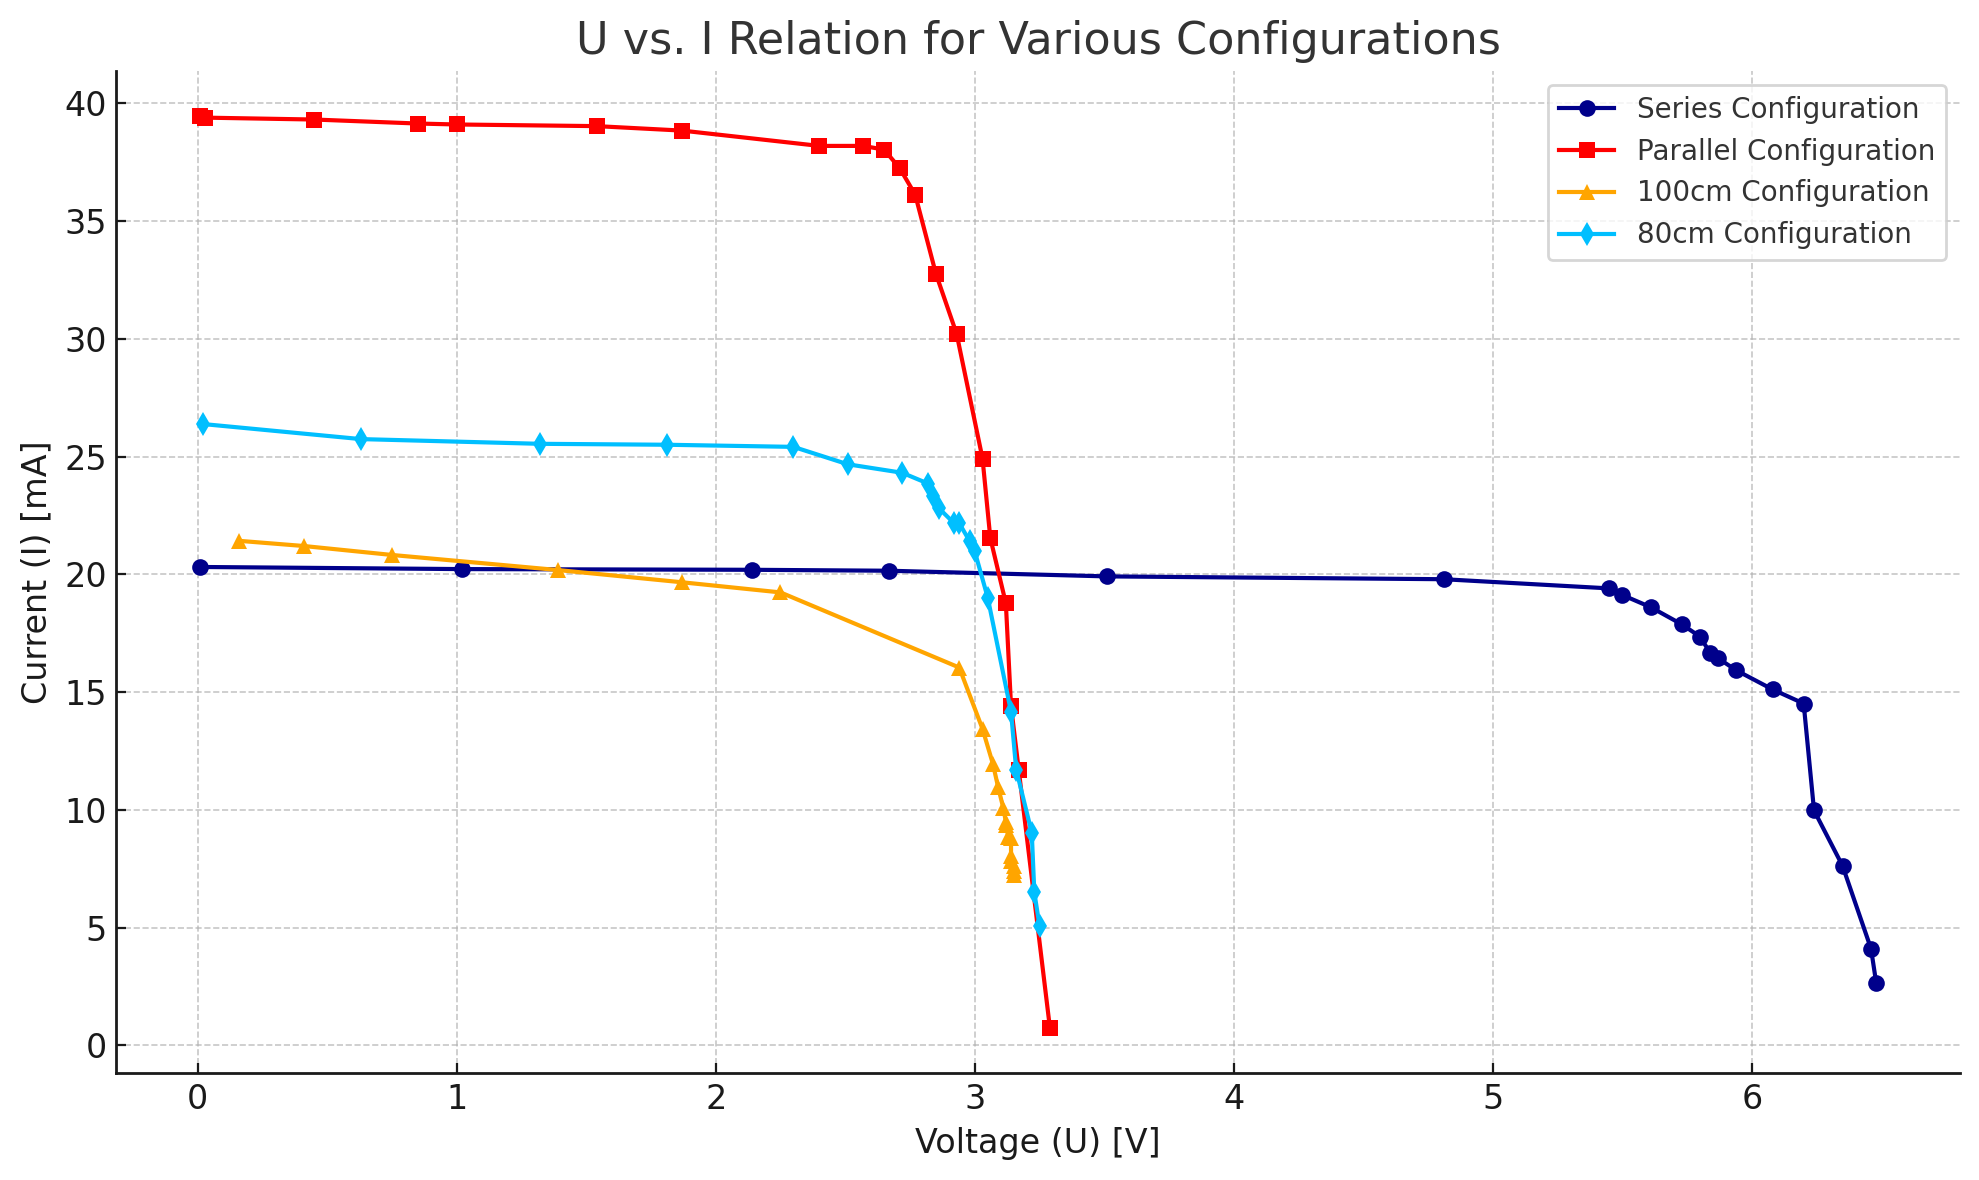
\includegraphics[width=0.9\textwidth]{output.png}
	\caption{I-V Relationship}
	\label{fig2}
\end{figure}

From this curve we see that the current and the voltage of solar cells show an inversely proportional trend.
To be more precise, this matches the equation we wanted to prove at the beginning of this report:
\begin{equation*}
	V = \frac{n k T}{q} \ln\left(\frac{I_{sc}}{I_0} + 1\right)
\end{equation*}

From the figure of series connection, we can clearly notice that the voltage is twice of the single cell connection while the current
remains unchanged. And for the parellel connection, the current was doubled while the volatge remains the same. Both connection methods 
meet the equation we would like to do handwaving proof.

\section{Conclusions and discussion}
\subsection{Conclusions}
\indent

In this experiment, we focused on the relationship, or say the I-V characteristics of solar cells. We first
measured the power of the light source which acted as the sun, and thet take down the data of different light source
situations for later analysis. Based on the results acquired from the experiment, we can say that we partly prove
the equation:
\begin{equation*}
	V = \frac{n k T}{q} \ln\left(\frac{I_{sc}}{I_0} + 1\right)
\end{equation*}

\subsection{Discussion}
\indent

There were also some potential errors in the experiment. For example, the time it took to measure all the data needed
for the lab report and following analysis is too long. During this period, the solar curve of the cells might 
change dramatically due to the high temperature generated by the lighy source. This can cause errors in the curves.
Also, the distance between the light and the cells are measured using a long ruler, which can be quite inaccurate.
This might also have some negative effects on the value of data we get.


\section{Works cited}
Department of Physics, Shanghai Jiaotong University, Exercise 3 (Solar Cells: I-V Characteristics) - lab manual [rev. 2.4], 2024\\
Python Software Foundation. (2020). Python Language Reference, version 3.9. Available at http://www.python.org\\
\\
All the figures displayed in the article (excluding the appendix) are given using Python 3.9.
\pagebreak
\appendix
\section{Datasheet}

\begin{figure}[htbp]
	\centering
	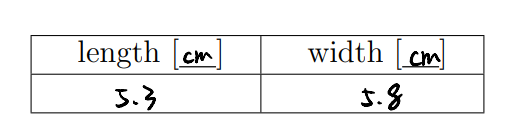
\includegraphics[width=0.75\textwidth]{D1.png}
	\caption{Datasheet 1}
\end{figure}

\begin{figure}[htbp]
	\centering
	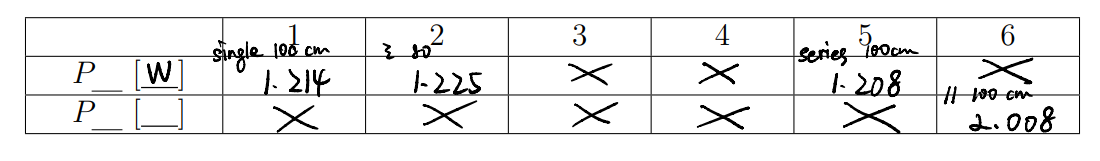
\includegraphics[width=0.75\textwidth]{D2.png}
	\caption{Datasheet 1}
\end{figure}

\begin{figure}[htbp]
	\centering
	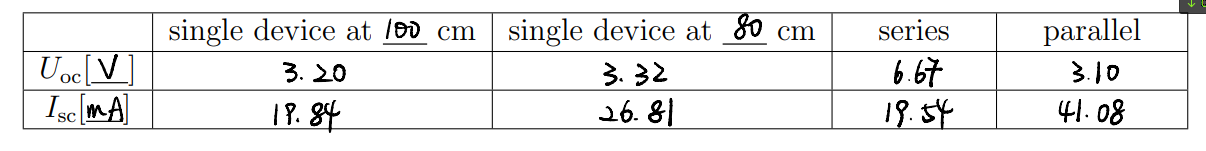
\includegraphics[width=0.75\textwidth]{D3.png}
	\caption{Datasheet 1}
\end{figure}

\begin{figure}[htbp]
	\centering
	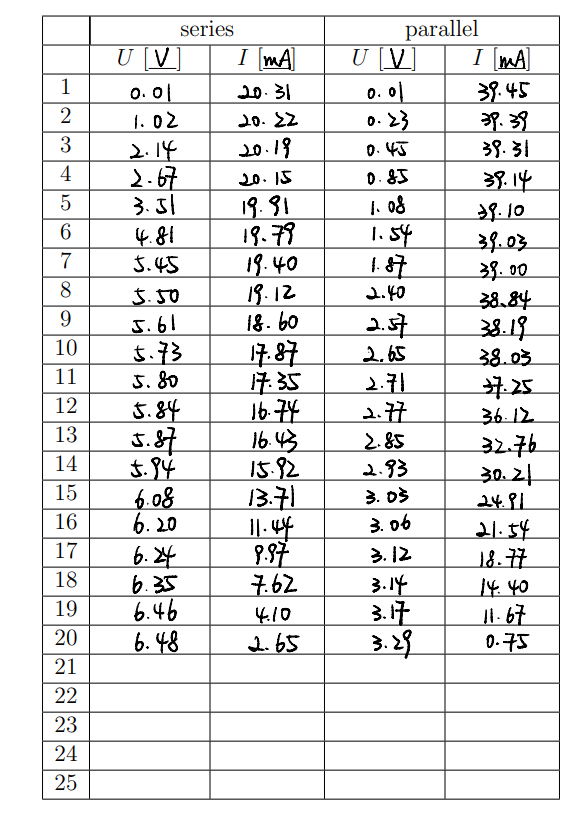
\includegraphics[width=0.75\textwidth]{D4.png}
	\caption{Datasheet 1}
\end{figure}

\begin{figure}[htbp]
	\centering
	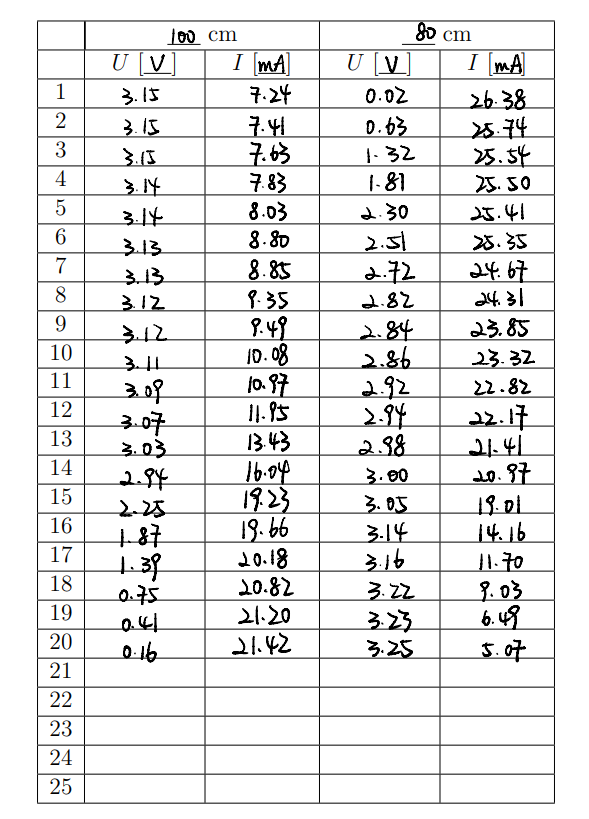
\includegraphics[width=0.75\textwidth]{D5.png}
	\caption{Datasheet 1}
\end{figure}


%\textcolor{blue}{Please remember to attach the original data sheet signed by your instructor.}
\end{document}